\section{Results}

Each subsection here is dedicated to a method and is accompanied with two confusion matrices for \tsne and PCA each. The matrix is from a single run of the model. Results were measured by running the model 100 times on different random splits of data which has been preprocessed with PCA methods discussed in implementation. From these runs we can extract the average accuracy and standard deviation for each model and determine the best one.

% macro for two-up figures, a few too many arguments maybe but will work.
% twoupfigure{img1}{img2}{caption main}{caption1}{caption2}{label}
\begin{figure}
    \centering
    \begin{subfigure}[b]{0.22\textwidth}
        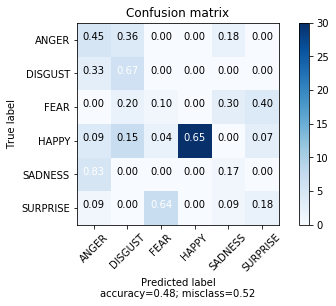
\includegraphics[width=\textwidth]{figures/pca-knn.png}
        \caption{\knn}
        \label{fig:pca-knn}
    \end{subfigure}
    \begin{subfigure}[b]{0.22\textwidth}
        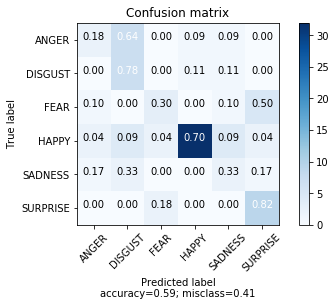
\includegraphics[width=\textwidth]{figures/pca-rf.png}
        \caption{RF}
        \label{fig:pca-rf}
    \end{subfigure}
    \begin{subfigure}[b]{0.22\textwidth}
        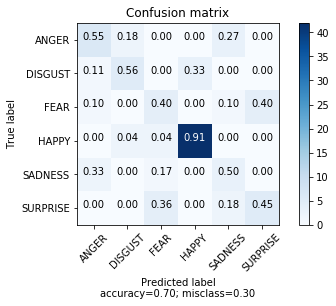
\includegraphics[width=\textwidth]{figures/pca-mlp.png}
        \caption{MLP}
        \label{fig:pca-mlp}
    \end{subfigure}
    \begin{subfigure}[b]{0.22\textwidth}
        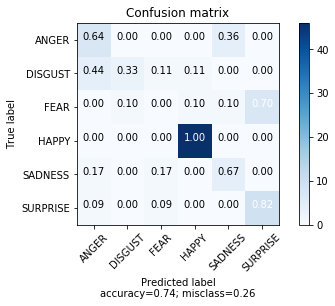
\includegraphics[width=\textwidth]{figures/pca-svm.png}
        \caption{SVM}
        \label{fig:pca-svm}
    \end{subfigure}
    \caption{Confusion matrices for methods run with PCA dimensionality reduction.}\label{fig:results}
\end{figure}

\subsection{\knn}

With \knn methods we can attain an average accuracy of $46.5\%$ with a standard deviation of $0.045$; this is a mediocre score. This difference in accuracy compared to other methods can be thought of as a problem with clustering and the nature of the landmark points. Any set of emotions where, for example, an eyebrow point is more or less the same point (e.g. surprised and happy), will be classified by kNN as the same emotion, no other points will be taken into account. Among our labels are two super-categories of emotions, positive (happy, surprised) and negative (fear, angry, disgust, sad). The reader is invited to make those emotions with his or her face and take note the placement of their eyebrows. They may notice they are in the same place for each emotion, other features may be in the same place too.

We ran another experiment to demonstrate that \knn can detect these distinctions. Simply by running the dataset through the \knn classifier and counting how many positive and negative emotions it accurately detects. The results are telling, we can classify positive emotions with 67\% accuracy and negative emotions with 89\% accuracy. We can inspect this further by referring to the relevant confusion matrix (figure \ref{fig:pca-knn}), \knn has quite admonishable accuracy when trying to classify the positive emotion surprise.

\subsection{Random Forests}

With RF methods we can attain an accuracy of $62.9\%$ with a standard deviation of $0.043$. While consistent, compared to the worst of our supervised methods it is still about 10\% less accurate. Furthermore, unlike \knn methods, RF's inherit structure determines features to be correlated, it is not just a series of points which some method is blindly clustering, hence the 15\% accuracy boost over \knn. An interesting difference to point out in the results is while \knn most misclassifies surprise, RF misclassifies anger as disgust (figure \ref{fig:pca-rf}). It is also worthwhile noting that RF is the best method with \tsne, although the accuracy is only barely better than random classification at 28\%.

\subsection{MLP}

With MLP methods we can attain an accuracy of $73.3\%$ with a standard deviation of $0.037$. This immediate increase in accuracy can demonstrate the advantages of fully using labels in a dataset. Unlike \knn methods, neural networks can fit correlations and relations in datasets, although perhaps over-fit in some places. After a closer look at the confusion matrix in figure \ref{fig:pca-mlp} we see a faint bottom-left to top-right diagonal from anger to sadness consisting of commonly misclassified emotions.

\subsection{SVM}

With SVM methods we get an accuracy of $74.00\%$ with a standard deviation of $0.045$. To a marginal detriment of consistency against MLP methods, this makes it the most accurate model. It is also the only model to score 100\% for a single emotion "happy". However, along with MLP methods, it misclassifies fear for surprise quite often (figure \ref{fig:pca-svm}).

% this part belongs somewhere else, could be quantified a bit more, like actually measuring distances from emotions.
By inspecting which emotions are most misclassified as others across all PCA figures for each classifier we can intuitively create an emotional spectrum (figure \ref{fig:spectrum}).

\begin{figure}
\centering
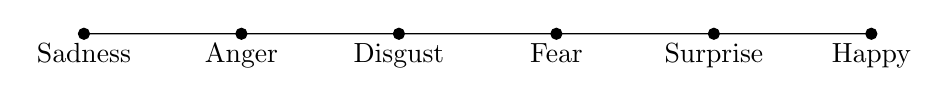
\begin{tikzpicture}[]
\filldraw
(0,0)  circle (2pt) node[align=left,   below] {Sadness}  --
(2,0)  circle (2pt) node[align=center, below] {Anger}    --
(4,0)  circle (2pt) node[align=center, below] {Disgust}  --
(6,0)  circle (2pt) node[align=center, below] {Fear}     --
(8,0)  circle (2pt) node[align=center, below] {Surprise} --
(10,0) circle (2pt) node[align=right,  below] {Happy};
\end{tikzpicture}
\caption{A spectrum of emotions inferred from confusion matrices.}
\label{fig:spectrum}
\end{figure}
